\chapter{Local Source Terms}
\label{Sec:source terms}

The \code{physics/sourceTerms} organizational directory contains several units 
that implement forcing terms.  The \code{Burn}, \code{Stir}, \code{Ionize}, and
\code{Diffuse} units contain implementations in \flashx.  Two other units,
\code{Cool} and \code{Heat}, contain only stub level routines in their API.

\section{Burn Unit}
\label{Sec:burn}

The nuclear burning implementation of the \code{Burn} unit uses a
sparse-matrix semi-implicit ordinary differential equation (ODE)
solver to calculate the nuclear burning rate and to update the fluid
variables accordingly (Timmes 1999). The primary interface routines
for this unit are \api{physics/sourceTerms/Burn/Burn_init}, which
sets up the nuclear isotope tables needed by the
unit, and \api{physics/sourceTerms/Burn/Burn}, which
calls the ODE solver and updates the hydrodynamical variables in a
single row of a single block.
The routine \api{physics/sourceTerms/Burn/Burn_computeDt} may limit the computational timestep because of burning considerations.
There is also a helper routine \code{Simulation/\-SimulationComposition/\-Simulation_initSpecies}
(see \api{Simulation/Simulation_initSpecies})
which provides the properties of ions included in the burning network.


\begin{comment}
% \begin{table}
% \caption{ \label{Tab:burn parameters} Runtime parameters used with the
% \code{Burn} unit.}
% \begin{center}
% \begin{tabular}{lllp{3.5in}}
% Variable    & Type      & Default   & Description\\
% \hline
% \code{algebra}         & integer   & 1 & Choice of linear algebra package for sparse matrices \\
% \code{enucDtFactor}    & real      & $1.0\times10^30$ & Time step limiter based on energy generation from burning \\
% \code{nuclearTempMin}  & real      & $1.1\times10^8$ & Minimum temperature in K    for burning to be allowed\\
% \code{nuclearTempMax}  & real      & $1.0\times10^{12}$
%                           & Maximum temperature in K   for burning to be allowed\\
% \code{nuclearDensMin}  & real      & $1.0\times10^{-10}$
%                           & Minimum    density (g~cm$^{-3}$) for burning to be allowed\\
% \code{nuclearDensMax}  & real      & $1.0\times10^{14}$
%                           & Maximum  density (g~cm$^{-3}$) for  burning to be allowed\\
% \code{nuclearNI56Max}  & real      & 0.4         & Maximum Ni$^{56}$ mass
%                             fraction for burning                    to be allowed\\
% \code{odeStepper}      & integer   & 1 & Choice of implicit integration scheme for evolving reaction network\\
% \code{useBurnTable}    & boolean   & false & Evaluate reaction rates directly, or by using a table approximation \\
% \code{useShockBurning} & boolean   & ?? & ?? \\
% \hline
% \end{tabular}
% \end{center}
% \end{table}
\end{comment}

\subsection{Algorithms}

~Modeling thermonuclear flashes typically requires the energy
generation rate due to nuclear burning over a large range of
temperatures, densities and compositions. The average energy generated
or lost over a period of time is found by integrating a system of
ordinary differential equations (the nuclear reaction network) for the
abundances of important nuclei and the total energy release.  In some
contexts, such as supernova models, the abundances themselves
are also of interest. In either case, the coefficients that appear in
the equations are typically extremely sensitive to temperature.  The
resulting stiffness of the system of equations requires the use of an
implicit time integration scheme.

A user can choose between two implicit integration methods and two
linear algebra packages in Flash-X. The runtime parameter
\rpi{Burn/odeStepper}
controls which integration method is used in the simulation. The
choice \code{odeStepper = 1} is the default and invokes a
Bader-Deuflhard scheme.  The choice \code{odeStepper = 2} invokes a
Kaps-Rentrop or Rosenbrock scheme.
The runtime parameter \rpi{Burn/algebra} controls which
linear algebra package is used in the simulation.  The choice
\code{algebra = 1} is the default and invokes the sparse matrix MA28 package.
The choice \code{algebra = 2} invokes the GIFT linear algebra routines.
While any combination of the integration methods and linear algebra
packages will produce correct answers, some combinations may execute
more efficiently than others for certain types of
simulations.  No general rules have been found for best combination
for a given simulation. The most efficient combination depends on the
timestep being taken, the spatial resolution of the model, the values
of the local thermodynamic variables, and the composition. Users are
advised to experiment with the various combinations to determine the
best one for their simulation.  However, an extensive analysis was performed in
the Timmes paper cited below.

Timmes (1999) reviewed several methods for solving stiff nuclear
reaction networks, providing the basis for the reaction network solvers
included with Flash-X.  The scaling properties and behavior of three
semi-implicit time integration algorithms (a traditional first-order
accurate Euler method, a fourth-order accurate Kaps-Rentrop / Rosenbrock method,
and a variable order Bader-Deuflhard method) and eight linear algebra
packages (LAPACK, LUDCMP, LEQS, GIFT, MA28, UMFPACK, and Y12M) were
investigated by running each of these 24 combinations on seven
different nuclear reaction networks (hard-wired 13- and 19-isotope
networks and soft-wired networks of 47, 76, 127, 200, and 489
isotopes).  Timmes' analysis suggested that the best balance of
accuracy, overall efficiency, memory footprint, and ease-of-use was
provided by the two integration methods (Bader-Deuflhard and Kaps-Rentrop)
and the two linear algebra packages (MA28 and GIFT) that are provided
with the Flash-X code.


\subsection{Reaction networks}


We begin by describing the equations solved by the nuclear burning
unit. We consider material that may be described by a density
$\rho$ and a single temperature $T$ and contains a number of isotopes
$i$, each of which has $Z_{i}$ protons and $A_i$ nucleons (protons +
neutrons). Let $n_i$ and $\rho_i$ denote the number and mass density,
respectively, of the $i$th isotope, and let $X_i$ denote its mass
fraction, so that
\begin{equation}
X_i = \rho_i/\rho = n_i A_i/(\rho N_A)\ ,
\end{equation}
where $N_A$ is Avogadro's number.
Let the molar abundance of
the $i$th isotope be
\begin{equation}
Y_i = X_i/A_i = n_i/(\rho N_A)\ .
\end{equation}
Mass conservation is then expressed by
\begin{equation}
\label{Eqn:mass conservation}
\sum_{i=1}^N X_i = 1~.
\end{equation}
At the end of each timestep, Flash-X checks that the stored abundances
satisfy \eqref{Eqn:mass conservation} to machine precision in order
to avoid the unphysical buildup (or decay) of the abundances or
energy generation rate. Roundoff errors in this equation can lead to
significant problems in some contexts (\eg, classical nova
envelopes), where trace abundances are important.

The general continuity equation for the $i$th isotope is given in
Lagrangian formulation by
\begin{equation}
\label{Eqn:isotope continuity}
\drvf {Y_i} {t} + \nabla \cdot \left ( Y_i \avec {V}_i \right ) = \dt {R_i}\ .
\end{equation}
In this equation
$\dt {R_i}$ is the total reaction rate due to
all binary reactions of the form {\it i(j,k)l},
\begin{equation}
\label{Eqn:binary rate}
\dt {R_{i}}
 = \sum_{j,k}
              Y_{l} Y_{k} \lambda _{kj}(l)  - Y_{i} Y_{j} \lambda _{jk}(i)\ ,
\end{equation}
where $\lambda _{kj}$ and $\lambda _{jk}$ are the reverse (creation)
and forward (destruction) nuclear reaction rates, respectively.
Contributions from three-body reactions, such as the triple-$\alpha$
reaction, are easy to append to \eqref{Eqn:binary rate}.  The mass
diffusion velocities $\avec{V}_i$ in \eqref{Eqn:isotope continuity}
are obtained from the solution of a multicomponent diffusion
equation (Chapman \& Cowling 1970; Burgers 1969; Williams 1988) and
reflect the fact that mass diffusion processes arise from pressure,
temperature, and/or abundance gradients as well as from external
gravitational or electrical forces.

The case $\avec{V}_i\equiv 0$ is important for two reasons. First,
mass diffusion is often unimportant when compared to other transport
processes, such as thermal or viscous diffusion (\ie, large Lewis
numbers and/or small Prandtl numbers). Such a situation obtains, for
example, in the study of laminar flame fronts propagating through
the quiescent interior of a white dwarf. Second, this case permits
the decoupling of the reaction network solver from the
hydrodynamical solver through the use of operator splitting, greatly
simplifying the algorithm.  This is the method used by the default
Flash-X distribution. Setting $\avec{V}_i\equiv 0$ transforms
\eqref{Eqn:isotope continuity} into
\begin{equation}
\label{Eqn:nucrate 1}
\drvf {Y_i} {t} = \dt {R_i}\ ,
\end{equation}
which may be written in the more compact, standard form
\begin{equation}
\label{Eqn:nucrate 2}
\dot {{\bf y}} = {\bf f} \ ({\bf y})\ .
\end{equation}
Stated another way, in the absence of mass diffusion or advection,
any changes to the fluid composition are due to local processes.

Because of the highly nonlinear temperature dependence of the
nuclear reaction rates and because the abundances themselves often
range over several orders of magnitude in value, the values of the
coefficients which appear in \eqref{Eqn:nucrate 1} and
\eqref{Eqn:nucrate 2} can vary quite significantly.  As a result,
the nuclear reaction network equations are ``stiff.'' A system of
equations is stiff when the ratio of the maximum to the minimum
eigenvalue of the Jacobian matrix ${\tilde {\bf
J}}\equiv\partial{{\bf f}}/\partial{{\bf y}}$ is large and
imaginary. This means that at least one of the isotopic abundances
changes on a much shorter timescale than another.  Implicit or
semi-implicit time integration methods are generally necessary to
avoid following this short-timescale behavior, requiring the
calculation of the Jacobian matrix.

It is instructive at this point to look at an example of how
\eqref{Eqn:nucrate 1} and the associated Jacobian matrix are
formed. Consider the $^{12}$C($\alpha$,$\gamma$)$^{16}$O reaction,
which competes with the triple-$\alpha$ reaction during helium
burning in stars. The rate $R$ at which this reaction proceeds is
critical for evolutionary models of massive stars, since it
determines how much of the core is carbon and how much of the core
is oxygen after the initial helium fuel is exhausted.  This reaction
sequence contributes to the right-hand side of \eqref{Eqn:nucrate
2} through the terms
\begin{eqnarray}
\nonumber
\dot {Y} (^4He)   & =& - Y(^4He) \ Y(^{12}C) \ R + \ldots \\
\dot {Y} (^{12}C) & =& - Y(^4He) \ Y(^{12}C) \ R \ + \ldots  \\
\nonumber
\dot {Y} (^{16}O) & =& + Y(^4He) \ Y(^{12}C) \ R \ + \ldots ,
\end{eqnarray}
where the ellipses indicate additional terms coming from other
reaction sequences.  The minus signs indicate that helium and carbon
are being destroyed, while the plus sign indicates that oxygen is
being created. Each of these three expressions contributes two terms
to the Jacobian matrix
${\tilde {\bf J}}$=$\partial{{\bf f}}/\partial{{\bf y}}$
\begin{eqnarray}
\nonumber
J(^4He,^4He)     = - Y(^{12}C) \ R \ + \ldots  \hskip 0.5in
&
J(^4He,^{12}C)   = - Y(^4He) \ R \ + \ldots \\
J(^{12}C,^4He)   = - Y(^{12}C) \ R \ + \ldots \hskip 0.5in
&
J(^{12}C,^{12}C) = - Y(^4He) \ R \ + \ldots   \\
\nonumber
J(^{16}O,^4He)   = + Y(^{12}C) \ R \ + \ldots \hskip 0.5in
&
J(^{16}O,^{12}C) = + Y(^4He) \ R \ + \ldots .
\end{eqnarray}
Entries in the Jacobian matrix represent the flow, in number of nuclei
per second, into (positive) or out of (negative) an isotope.  All of the
temperature and density dependence is included in the reaction rate
$R$.  The Jacobian matrices that arise from nuclear reaction networks
are neither positive-definite nor symmetric, since the forward and
reverse reaction rates are generally not equal. In addition, the
magnitudes of the matrix entries change as the abundances,
temperature, or density change with time.

This release of \flashx contains three reaction networks.
A seven-isotope alpha-chain (\code{Iso7}) is useful for problems that
do not have enough memory to carry a larger set of isotopes.
The 13-isotope $\alpha$-chain plus heavy-ion reaction network (\code{Aprox13})
is suitable for most multi-dimensional simulations of stellar phenomena,
where having a reasonably accurate energy generation rate is of primary
concern.  The 19-isotope reaction network (\code{Aprox19}) has the same
$\alpha$-chain and heavy-ion reactions as the 13-isotope network, but it
includes additional isotopes to accommodate some types of hydrogen burning
(PP chains and steady-state CNO cycles), along with some aspects of
photo-disintegration into $^{54}$Fe. This 19 isotope reaction network
is described in Weaver, Zimmerman, \& Woosley (1978).

%The \code{Ppcno}
%network includes reactions for the pp and CNO cycles.  A number of simple
%single-reaction networks are also provided.

The networks supplied with Flash-X are examples of a ``hard-wired'' reaction
network, where each of the reaction sequences are carefully entered
by hand.  This approach is suitable for small networks, when minimizing
the CPU time required to run the reaction network is a primary
concern, although it suffers the disadvantage of inflexibility.



\subsubsection{Two linear algebra packages:  MA28 and GIFT}

As mentioned in the previous section, the Jacobian matrices of
nuclear reaction networks tend to be sparse, and they become more
sparse as the number of isotopes increases.  Since implicit or
semi-implicit time integration schemes generally require solving
systems of linear equations involving the Jacobian matrix, taking
advantage of the sparsity can significantly reduce the CPU time
required to solve the systems of linear equations.

The MA28 sparse matrix package used by Flash-X is described by Duff,
Erisman, \& Reid (1986).  This package, which has been described
as the ``Coke classic'' of sparse linear algebra packages, uses a direct
-- as opposed to an iterative -- method for solving linear systems.  Direct
methods typically divide the solution of $\tilde{{\bf A}} \cdot {\bf
x} = {\bf b}$ into a symbolic LU decomposition, a numerical LU
decomposition, and a backsubstitution phase.  In the symbolic LU
decomposition phase, the pivot order of a matrix is determined, and a
sequence of decomposition operations that minimizes the amount of
fill-in is recorded. Fill-in refers to zero matrix elements which
become nonzero (\eg, a sparse matrix times a sparse matrix is
generally a denser matrix).  The matrix is not decomposed; only the
steps to do so are stored. Since the nonzero pattern of a chosen
nuclear reaction network does not change, the symbolic LU
decomposition is a one-time initialization cost for reaction networks.
In the numerical LU decomposition phase, a matrix with the same pivot
order and nonzero pattern as a previously factorized matrix is
numerically decomposed into its lower-upper form.  This phase must be
done only once for each set of linear equations.  In the
backsubstitution phase, a set of linear equations is solved with the
factors calculated from a previous numerical decomposition.  The
backsubstitution phase may be performed with as many right-hand sides
as needed, and not all of the right-hand sides need to be known in
advance.

MA28 uses a combination of nested dissection and frontal envelope
decomposition to minimize fill-in during the factorization stage.  An
approximate degree update algorithm that is much faster
(asymptotically and in practice) than computing the exact degrees is
employed.  One continuous real parameter sets the amount of searching
done to locate the pivot element. When this parameter is set to zero,
no searching is done and the diagonal element is the pivot, while when
set to unity, partial pivoting is done.  Since the matrices
generated by reaction networks are usually diagonally dominant, the
routine is set in Flash-X to use the diagonal as the pivot
element. Several test cases showed that using partial pivoting did not
make a significant accuracy difference but was less efficient, since
a search for an appropriate pivot element had to be performed.  MA28
accepts the nonzero entries of the matrix in the \hbox{$(i, j,
a_{i,j}$)} coordinate system and typically uses 70$-$90\% less
storage than storing the full dense matrix.


GIFT is a program which generates Fortran subroutines for solving a
system of linear equations by Gaussian elimination (Gustafson,
Liniger, \& Willoughby 1970; M\"uller 1997).  The full matrix
$\tilde{{\bf A}}$ is reduced to upper triangular form, and
backsubstitution with the right-hand side {\bf b} yields the solution
to $\tilde{{\bf A}} \cdot {\bf x} = {\bf b}$.  GIFT generated routines
skip all calculations with matrix elements that are zero; in this
restricted sense, GIFT generated routines are sparse, but the storage
of a full matrix is still required.  It is assumed that the pivot
element is located on the diagonal and no row or column interchanges
are performed, so GIFT generated routines may become unstable if the
matrices are not diagonally dominant.  These routines must decompose
the matrix for each right-hand side in a set of linear equations.
GIFT writes out (in Fortran code) the sequence of Gaussian elimination
and backsubstitution steps without any do loop constructions on the matrix
$A(i,j)$. As a result, the routines generated by GIFT can be quite
large. For the 489 isotope network discussed by Timmes (1999), GIFT
generated $\sim$ 5.0$\times$10$^7$ lines of code! Fortunately, for
small reaction networks (less than about 30 isotopes), GIFT generated
routines are much smaller and generally faster than other linear
algebra packages.


The Flash-X runtime parameter \rpi{Burn/algebra} controls
which linear algebra package is used in the simulation.  \code{algebra = 1}
is the default choice and invokes the sparse matrix MA28 package.
\code{algebra = 2} invokes the GIFT linear algebra routines.





\subsubsection{Two time integration methods}


One of the time integration methods used by Flash-X for evolving the
reaction networks is a 4th-order accurate Kaps-Rentrop, or Rosenbrock method. In
essence, this method is an implicit Runge-Kutta algorithm.  The
reaction network is advanced over a timestep $h$ according to
\begin{equation}
\label{Eqn:kr1}
{\bf y}^{n+1} = {\bf y}^n + \sum_{i=1}^4 b_i \Delta_i
\ ,
\end{equation}
where the four vectors $\Delta^i$ are found from successively
solving the four matrix equations

\begin{eqnarray}
(\tilde{{\bf 1}}/\gamma h - \tilde{{\bf J}}) \cdot \Delta_1 & = &
{\bf f} ({\bf y}^n)\\
(\tilde{{\bf 1}}/\gamma h - \tilde{{\bf J}}) \cdot \Delta_2 & = &
{\bf f} ({\bf y}^n + a_{21}\Delta_1) + c_{21}\Delta_1/h\\
(\tilde{{\bf 1}}/\gamma h - \tilde{{\bf J}}) \cdot \Delta_3 & = &
{\bf f} ({\bf y}^n + a_{31}\Delta_1 + a_{32}\Delta_2) +
(c_{31}\Delta_1 + c_{32}\Delta_2)/h\\
(\tilde{{\bf 1}}^\gamma h - \tilde{{\bf J}}) \cdot \Delta_4 & = &
{\bf f} ({\bf y}^n + a_{31}\Delta_1 + a_{32}\Delta_2) +
(c_{41}\Delta_1 + c_{42}\Delta_2 + c_{43}\Delta_3)/h
\ .
\end{eqnarray}
$b_i$, $\gamma$, $a_{ij}$, and $c_{ij}$ are
fixed constants of the method.  An estimate of the accuracy of the
integration step is made by comparing a third-order solution with a
fourth-order solution, which is a significant improvement over the
basic Euler method.  The minimum cost of this method $-$ which applies
for a single timestep that meets or exceeds a specified integration
accuracy $-$ is one Jacobian evaluation, three evaluations of the
right-hand side, one matrix decomposition, and four backsubstitutions.
Note that the four matrix equations represent a staged set of linear equations
($\Delta_4$ depends on $\Delta_3 \ldots$ depends on $\Delta_1$).  Not
all of the right-hand sides are known in advance. This general feature
of higher-order integration methods impacts the optimal choice of a
linear algebra package.  The fourth-order Kaps-Rentrop routine in
Flash-X makes use of the routine GRK4T given by Kaps \& Rentrop
(1979).

Another time integration method used by Flash-X for evolving the reaction
networks is the variable order Bader-Deuflhard method (\eg, Bader \&
Deuflhard 1983).  The reaction network is advanced
over a large timestep $H$ from ${\bf y}^n$ to ${\bf y}^{n+1}$ by the
following sequence of matrix equations. First,
\begin{eqnarray}
\nonumber
h & = & H/m \\
\label{Eqn:BD 1}
(\tilde{{\bf 1}} - \tilde{{\bf J}}) \cdot \Delta_0 & = & h {\bf f}
({\bf y}^n) \\
\nonumber
{\bf y}_1 & = &{\bf y}^n + \Delta_0\ .
\end{eqnarray}
Then from $k=1,2,\ldots,m-1$
\begin{eqnarray}
\nonumber
(\tilde{{\bf 1}} - \tilde{{\bf J}}) \cdot {\bf x} & = &
h {\bf f}({\bf y}_{k}) - \Delta_{k-1}  \\
\Delta_k & = & \Delta_{k-1} + 2 {\bf x} \\
\nonumber
{\bf y}_{k+1} & = &{\bf y}_k + \Delta_k \ ,
\end{eqnarray}
and closure is obtained by the last stage
\begin{eqnarray}
\nonumber
(\tilde{{\bf 1}} - \tilde{{\bf J}}) \cdot \Delta_m & = &
h [ {\bf f} ({\bf y}_m)  - \Delta_{m-1} ] \\
\label{Eqn:BD 3}
{\bf y}^{n+1} & = &{\bf y}_m + \Delta_m \ .
\end{eqnarray}
This staged sequence of matrix equations is executed at least twice
with $m=2$ and $m=6$, yielding a fifth-order method.  The sequence
may be executed a maximum of seven times, which yields a
fifteenth-order method.  The exact number of times the staged
sequence is executed depends on the accuracy requirements (set to
one part in 10$^6$ in Flash-X) and the smoothness of the solution.
Estimates of the accuracy of an integration step are made by
comparing the solutions derived from different orders.  The minimum
cost of this method --- which applies for a single timestep that met
or exceeded the specified integration accuracy --- is one Jacobian
evaluation, eight evaluations of the right-hand side, two matrix
decompositions, and ten backsubstitutions.  This minimum cost can be
increased at a rate of one decomposition (the expensive part) and
$m$ backsubstitutions (the inexpensive part) for every increase in
the order $2k+1$. The cost of increasing the order is compensated
for, hopefully, by being able to take correspondingly larger (but
accurate) timestep.  The controls for order versus step size are a
built-in part of the Bader-Deuflhard method.  The cost per step of
this integration method is at least twice as large as the cost per
step of either a traditional first-order accurate Euler method or
the fourth-order accurate Kaps-Rentrop discussed above. However, if
the Bader-Deuflhard method can take accurate timesteps that are at
least twice as large, then this method will be more efficient
globally. Timmes (1999) shows that this is typically (but not
always!) the case. Note that in \eqnsref{Eqn:BD 1}{Eqn:BD 3}, not
all of the right-hand sides are known in advance, since the sequence
of linear equations is staged. This staging feature of the
integration method may make some matrix packages, such as MA28, a
more efficient choice.


The Flash-X runtime parameter \rpi{Burn/odeStepper}
controls which integration method is used in the simulation. The choice
\code{odeStepper = 1} is the default and invokes the variable order
Bader-Deuflhard scheme.  The choice \code{odeStepper = 2} invokes the
fourth order Kaps-Rentrop / Rosenbrock scheme.

\subsection{Detecting shocks}

For most astrophysical detonations, the shock structure is so thin
that there is insufficient time for burning to take place within the
shock.  However, since numerical shock structures tend to be much
wider than their physical counterparts, it is possible for a significant
amount of burning to occur within the shock.  Allowing this to happen
can lead to unphysical results.  The burner unit includes a
multidimensional shock detection algorithm that can be used to prevent
burning in shocks.  If the \rpi{Burn/useShockBurn} parameter is set to
\code{.false.}, this algorithm is used to detect shocks in the
Burn unit and to switch off the burning in shocked
cells.

Currently, the shock detection algorithm supports Cartesian and 2-dimensional
cylindrical coordinates.  The basic algorithm is to compare the jump
in pressure in the direction of compression (determined by looking at
the velocity field) with a shock parameter (typically 1/3).  If the
total velocity divergence is negative and the relative pressure jump
across the compression front is larger than the shock parameter, then
a cell is considered to be within a shock.

This computation is done on a block by block basis.  It is important
that the velocity and pressure variables have up-to-date guard cells,
so a guard cell call is done for the burners only if we are detecting
shocks ({\it i.e.} \code{useShockBurning = .false.}).


\subsection{Energy generation rates and reaction rates}

The instantaneous energy generation rate is given by the sum
\begin{equation}
\dot {\epsilon}_{\rm nuc} = N_A \ \sum_i \ \drvf {Y_{i}} {t} \ .
\end{equation}
Note that a nuclear reaction network does not need to be evolved in
order to obtain the instantaneous energy generation rate, since only
the right hand sides of the ordinary differential equations need to be
evaluated. It is more appropriate in the Flash-X program to use the
average nuclear energy generated over a timestep
\begin{equation}
\dot {\epsilon}_{\rm nuc} = N_A \ \sum_i \ {\Delta Y_i \over \Delta t}\ .
\end{equation}
In this case, the nuclear reaction network does need to be evolved.
The energy generation rate, after subtraction of any neutrino losses,
is returned to the Flash-X program for use with the operator splitting
technique.

The tabulation of Caughlan \& Fowler (1988) is used in Flash-X for most
of the key nuclear reaction rates.  Modern values for some of the
reaction rates were taken from the reaction rate library of Hoffman
(2001, priv.\ comm.).  A user can choose between two reaction rate
evaluations in Flash-X.  The runtime parameter \rpi{Burn/useBurnTable} controls
which reaction rate evaluation method is used in the simulation. The
choice \code{useBurnTable = 0} is the default and evaluates the
reaction rates from analytical expressions.  The choice \code{useBurnTable =
1} evaluates the reactions rates from table interpolation. The
reaction rate tables are formed on-the-fly from the analytical
expressions.  Tests on one-dimensional detonations and hydrostatic
burnings suggest that there are no major differences in the abundance
levels if tables are used instead of the analytic expressions; we find
less than 1\% differences at the end of long timescale runs.  Table
interpolation is about 10 times faster than evaluating the analytic
expressions, but the speedup to Flash-X is more modest, a few percent at
best, since reaction rate evaluation never dominates in a real
production run.

Finally, nuclear reaction rate screening effects as formulated by
Wallace {\it et al.} (1982) and decreases in the energy generation rate
$\dot {\epsilon}_{\rm nuc}$ due to neutrino losses as given by Itoh {\it et
al.} (1996) are included in Flash-X.

\subsection{Temperature-based timestep limiting}

When using explicit hydrodynamics methods, a timestep
limiter must be used to ensure the stability of the numerical solution.
The standard CFL limiter is always used when an explicit hydrodynamics
unit is included in Flash-X.  This constraint does not allow any
information to travel more than one computational cell per timestep.
When coupling burning with the hydrodynamics, the CFL timestep may be so
large compared to the burning timescales that the nuclear energy
release in a cell may exceed the existing internal energy in that
cell.  When this happens, the two operations (hydrodynamics and
nuclear burning) become decoupled.

% This enucDtFactor is supposed be less than 1 via the documentation.  But the CONFIG implies the
%  default is 1.0E+30.  Too much discrepancy to figure out now.
To limit the timestep when burning is performed, an additional constraint is imposed.   The limiter tries to force the energy generation from burning to be smaller than the internal energy in a cell.  The runtime parameter \rpi{Burn/enucDtFactor} controls this ratio.  The timestep limiter is calculated as
\begin{equation}
\Delta t_{burn} = \code{enucDtFactor} \cdot \frac{E_{int}}{E_{nuc}}
\end{equation}
where $E_{nuc}$ is the nuclear energy, expressed as energy per volume per time, and
$E_{int}$ is the internal energy per volume.
For good coupling between the hydrodynamics and burning,
\code{enucDtFactor} should be $< 1$. The default value is kept
artificially high so that in most simulations the time limiting due to
burning is turned off. Care must be exercised in the use of this routine.


\begin{comment} %this stuff all removed in flash3
To help fix this problem, the
timestep may be determined by the change in temperature in a cell.  Flash-X
includes a temperature based timestep limiter that tries to constrain
the change in temperature in a cell to be less than a user defined
parameter.  To use this limiter, set \code{itemp\_limit = 1} and
specify the fractional temperature change \rpi{Driver/temp_factor} you are
willing to tolerate.
\marginpar{Why is this RT parameter in Driver?}
While there is no guarantee that the temperature change
will be smaller than this, since the timestep was already taken by the time
this was computed, this method is successful in restoring coupling between
the hydrodynamics and burning operators.  This timestep will be computed as
\begin{equation}
\Delta t = \code{temp\_factor} \cdot \frac{T}{\Delta T} \cdot
{\Delta t_{old}}~,
 \end{equation}
where $\Delta t$ is the difference in the temperature of a cell from one
timestep to the next, and $\Delta t_{old}$ is the last timestep.  To prevent
the timestep from varying wildly from one step to the next, it is
useful to force the maximum change in timestep to be a small factor
over the previous one through the \rpi{Driver/tstep_change_factor}
parameter.
\end{comment}



\section{Ionization Unit}
\label{Sec:ionization}

The analysis of UV and X-ray observations, and in particular of
spectral lines, is a powerful diagnostic tool of the physical
conditions in  astrophysical plasmas (\eg, the outer layers of the
solar atmosphere, supernova remnants, \etc).  Since deviation from
equilibrium ionization may have a non-negligible effect on the UV and
X-ray lines, it is crucial to take into account these effects in the
modeling of plasmas and in the interpretation of the relevant
observations.

In light of the above observations, Flash-X contains the unit \code{Ionize},
in particular the implementation
\code{physics/\-source\-Terms/\-Ionize/\-Ionize\-Main/\-Nei}, which is capable of computing the
density of each ion species of a given element taking into account
non-equilibrium ionization (NEI). This is accomplished by solving a
system of equations consisting of the fluid equations of the whole
plasma and the continuity equations of the ionization species of the
elements considered.  The densities of the twelve most abundant
elements in astrophysical material (He, C, N, O, Ne, Mg, Si, S, Ar,
Ca, Fe, and Ni) plus fully ionized hydrogen and electrons can be
computed by this unit.

The Euler equations plus the set of advection equations for all the
ion species take the following form
\begin{eqnarray}
\label{Eqn:ioeuler1}
{{\partial \rho} \over {\partial t}}
 + {\bf \nabla} \cdot \left ( \rho {\bf v} \right ) & = & 0\\
{\partial \rho {\bf v} \over \partial t} +
 {\bf \nabla}  \cdot \left ( \rho {\bf v} {\bf v} \right ) +
 {\bf \nabla}  P
 & = & \rho {\bf g}\\
\label{Eqn:ioeuler3}
{\partial \rho E \over \partial t} +
 {\bf \nabla} \cdot \left [ \left ( \rho E + P \right ) {\bf v}
 \right ] & = &
 \rho {\bf v} \cdot {\bf g} \ \left  [\ +\ S\ \right ] \\
\label{Eqn:ioeuler4}
 {\partial n_i^Z \over \partial t} + {\bf \nabla} \cdot n_i^Z {\bf v}
& = & R_i^Z \ \ (i=0,\ldots,Z) \ ,
\end{eqnarray}
where $\rho$ is the fluid density, $t$ is the time, ${\bf v}$ is the
fluid velocity, $P$ is the pressure, $E$ is the sum of the internal
energy and kinetic energy per unit mass, ${\bf g}$ is the
acceleration due to gravity, $n_i^Z$ is the number density of ions
of ionization level $i$ of the element $Z$, 
and
\begin{equation}
R_i^Z = N_e[n_{i+1}^Z \alpha_{i+1}^Z + n_{i-1}^Z S_{i-1}^Z -
n_{i}^Z(\alpha_{i}^Z + S_{i}^Z)]~,
\end{equation}
where $N_e$ is the electron number density, $\alpha_{i}^Z \equiv
\alpha(N_e, T)$ are the coefficients of collisional and dielectronic recombination, 
and $S_i^Z \equiv S(N_e, T)$ are the collisional
ionization coefficients of Summers(1974).
Note that \code{NSPECIES}, the total number of Flash-X species, will be given by
$$ N_{\mathrm{spec}} = 2 + \sum_Z (Z+1) ;$$
the sum ranges over all the elements from the list above that are included
in the problem, and the additional $2$ comes from the hydrogen and electron mass
fractions which are automatically included by the \code{IonizeMain} \subunit.

\subsection{Algorithms}
A fractional step method is required to integrate the equations
and in particular to decouple the NEI solver from the hydro solver.
For each timestep, the homogeneous hydrodynamic transport equations
given by \eqref{Eqn:ioeuler1} are solved using the
Flash-X hydrodynamics solver with $R_i^Z=0$. After each transport step, the
``stiff'' systems  of ordinary differential equations (one system per element included in the simulation) for the NEI
problem
\begin{equation}
{\partial n_i^Z \over \partial t} = R_i^Z \ (i=0,\ldots,Z)
\end{equation}
are integrated.
This step incorporates the reactive source terms.  Within each grid cell, the
above equations can be solved separately with a standard ODE method.
Since this system is ``stiff'', it is solved using
the Bader-Deuflhard time integration solver
with the MA28 sparse matrix package.  Timmes (1999) has shown
that these two algorithms together provide the best balance of
accuracy and overall efficiency for the similar problem of
nuclear burning, see \secref{Sec:burn}.

Note that in the present version, the contribution of the ionization
and recombination to the energy equation (the bracketed term in
\eqref{Eqn:ioeuler3}) is not accounted for.  Also, it should be
noted that the source term in the NEI unit implementation is adequate to solve
the problem for optically thin plasma in the ``coronal''
approximation; just collisional ionization, auto-ionization,
radiative recombination, and dielectronic recombination are
considered.

\subsection{Usage}
\label{Sec:ionization usage}

In order to run a Flash-X executable that uses the ionization
unit, the ionization coefficients of Summers (1974) must be
contained in a file named \code{summers\_den\_1e8.rates} in the same
directory as the executable when the simulation is run.  This file
is copied into the \code{object/} directory
with the \code{Config} keyword \code{DATAFILES} in the
\code{physics/\-sourceTerms/\-Ionize/\-IonizeMain} implementation. 

The \code{Ionize} unit supplies the runtime
parameters described in \tblref{Tab:ioniz parameters}.
\begin{table} \caption{ Runtime
parameters used with the \code{Ionize} unit.}
\label{Tab:ioniz parameters}
\begin{center}
\begin{tabular}{lllp{3in}}

Variable        & Type          & Default & Description\\

\hline
\rpi{Ionize/tneimin} & real          & $1.0\times10^4$      &  Min nei temperature   \\
\rpi{Ionize/tneimax} & real          & $1.0\times10^7 $    & Max nei temperature\\
\rpi{Ionize/dneimin} & real          & $1.0$     & Min nei electron number
density\\
\rpi{Ionize/dneimax} & real          & $1.0\times10^{12}$     & Max nei electron number density\\

\hline
\end{tabular}
\end{center}
\end{table}
There are two implementations of
\code{physics/\-sourceTerms/\-Ionize/\-IonizeMain}: the default implementation,
\code{Nei} (tested using \code{Neitest} (see \secref{Sec:neitest})),
and \code{Eqi} (untested in \flashx).  The former computes ion species
for non-equilibrium ionization, and the latter computes ion species in
the approximation of ionization equilibrium.

The \code{Ionize} unit requires that the subunit implementation
\code{Simulation/\-SimulationComposition/\-Ionize} be used to set up
the ion species of the fluid.  The ions are defined in a file
\code{Simulation/\-Simulation\-Composition/\-Ionize/\-SpeciesList.txt},
however, the \code{Config} file in the simulation directory
(e.g. \code{Simulation/\-SimulationMain/\-Neitest/\-Config}) defines
which subset of these elements are to be used.
%There are several subunits that
%include all or a subset of the possible elements and the ions of
%those elements. \code{materials/composition/ioniz/all} includes all
%of the elements and is the default subunit.
%\code{materials/composition/C+O+Ca+Fe} includes carbon, oxygen,
%calcium and iron.  

%DEV CD: Its not actually this simple.  We have flexibility with the
%Simulation unit, but no flexibility in Ionize unit.

%To use the \code{Ionize} unit with a different
%subset of elements, a new SpeciesList.txt should be defined in the simulation's home directory.

%new subunit should be added to the
%compositions directory.  
%\secref{Sec:ioniz composition} describes
%how to create a new composition.


\section{Stir Unit}
\label{Sec:stir}

The addition of driving terms in a hydrodynamical simulation can
be a useful feature, for example, in generating turbulent flows or
for simulating the addition of power on larger scales (\eg, supernova
feedback into the interstellar medium).  The \unit{Stir}
unit comes in two implementations: 1) the \code{Generate} implementation, in which a divergence-free,
random time-correlated `stirring' velocity is directly added at selected modes in the
simulation and 2) the \code{FromFile} implementation, in which a stirring field
is set up from data residing on a file. The \code{FromFile} implementation allows to
set up identical stirring fields on different platforms, and thus comparisons
can be made between different codes.

Before Flash-X 4.2, the implementation now called \code{Generate} was 
the only one provided.  It is still the default that is being
used if one specifies just 
\begin{code}
  REQUIRES physics/sourceTerms/Stir
\end{code}
in a \code{Config} file or \code{-unit=physics/sourceTerms/Stir} on the 
\code{setup} command line.

\subsection{Stir Unit: Generate Implementation}
\label{Sec:stirgenerate}

In the generate implementation, the Stir unit directly adds a divergence-free, time-correlated
`stirring' velocity at selected modes in the simulation.

The time-correlation is important for modeling realistic driving
forces.   Most large-scale driving forces are time-correlated, rather
than white-noise; for instance, turbulent stirring from larger scales
will be correlated on timescales related to the lifetime of an eddy
on the scale of the simulation domain.  This time correlation
will lead to coherent structures in the simulation that will be
absent with white-noise driving.

For each mode at each timestep, six separate phases (real and
imaginary in each of the three spatial dimensions) are evolved by an
Ornstein-Uhlenbeck (OU) random process (Uhlenbeck 1930).   The OU process is a zero-mean,
constant-rms
process, which at each step `decays' the previous value by an exponential
$f = e^{(\frac{\Delta t}{\tau})}$ and then adds a Gaussian random variable with
a given variance, weighted by a 'driving' factor $\sqrt (1 - f^2)$.
Since the OU process represents a
velocity, the variance is chosen to be the square root of the specific
energy input rate (set by the runtime parameter \rpi{Stir/st\_energy})
divided by the decay time $\tau$ (\rpi{Stir/st\_decay}). In the limit that the
timestep $\Delta t \rightarrow 0$, it is easily seen that the algorithm
represents a linearly-weighted summation of the old state with the new
Gaussian random variable.

By evolving the phases of the stirring modes in Fourier space, imposing
a divergence-free condition is relatively straightforward.  At each
timestep, the solenoidal component of the velocities is projected out,
leaving only the non-compressional modes to add to the velocities.

The velocities are then converted to physical space by a direct Fourier
transform -- \ie, adding the $\sin$ and $\cos$ terms explicitly.
Since most drivings involve a fairly small number of modes,
this is more efficient than an FFT, since the FFT would need large
numbers of modes (equal to six times the number of cells in the domain),
the vast majority of which would have zero amplitude.

\subsection{Stir Unit: FromFile Implementation}
\label{Sec:stirfromfile}

In the from file implementation, the Stir unit sets up a stirring field from data residing on a file.
Here we summarize the method for driving turbulence used in Federrath et al.~(2010, A\&A, 512, A81).
Please refer to that paper for further details.

Turbulence decays in about a crossing time, because the kinetic energy carried by the turbulence
dissipates on small scales and turns into heat. In order to study the statistics of turbulence
(e.g., the PDF, power spectrum, structure functions, etc.) over a significant time period thus
requires continuous stirring (also called driving or forcing) with a turbulent acceleration field,
which we call $\vec{f}(\vec{x},t)$ in the following.

The stirring field $\vec{f}$ is often modeled with a spatially static pattern for which the amplitude
is adjusted in time. This results in a roughly constant energy input on large scales, but has the
disadvantage that the turbulence is not really random, because the large-scale pattern is fixed, which
may introduce undesirable systematics. Other studies model $\vec{f}$ such that it can vary in time
\emph{and} space to achieve a smoothly varying pattern that resembles the flow of kinetic energy from
scales larger than the simulation box scale. The most widely used method to achieve this is the
Ornstein-Uhlenbeck (OU) process. The OU process is a well-defined stochastic process with a finite
autocorrelation timescale. It can be used to excite turbulent motions in 3D, 2D, or 1D simulations
as explained in Eswaran \& Pope (1988, Computers \& Fluids, 16, 257).

The OU process is a stochastic differential equation describing the evolution of $\widehat{\vec{f}}$
in Fourier space ($k$-space):
\begin{equation} \label{eq:ou}
\mathrm{d}\widehat{\vec{f}}\,(\vec{k},t) = f_{0\,}(\vec{k})\;\mathcal{\underline{P}}^{\,\zeta}(\vec{k})\;
\mathrm{d}\mathcal{\vec{W}}(t)\,-\,\widehat{\vec{f}}\,(\vec{k},t)\,\frac{\mathrm{d}t}{T}\;.
\end{equation}
The first term on the right hand side is a diffusion term. This term is modeled by a Wiener process
$\mathcal{\vec{W}}(t)$, which adds a Gaussian random increment to the vector field given in the previous
time step $\mathrm{d}t$. Wiener processes are random processes, such that
\begin{equation}
\mathcal{\vec{W}}(t)-\mathcal{\vec{W}}(t-\mathrm{d}t)=\mathcal{\vec{N}}(0,\mathrm{d}t)\;,
\end{equation}
where $\mathcal{\vec{N}}(0,\mathrm{d}t)$ denotes the 3D, 2D, or 1D version of a Gaussian distribution
with zero mean and standard deviation $\mathrm{d}t$. This is combined with a projection using the
projection tensor $\mathcal{\underline{P}}^{\,\zeta}(\vec{k})$ in Fourier space. In index notation, the
projection operator reads
\begin{equation} \label{eq:projectionoperator}
\mathcal{P}_{ij}^\zeta\,(\vec{k}) = \zeta\,\mathcal{P}_{ij}^\perp\,(\vec{k})+(1-\zeta)\,
\mathcal{P}_{ij}^\parallel\,(\vec{k}) = \zeta\,\delta_{ij}+(1-2\zeta)\,\frac{k_i k_j}{|k|^2}\;,
\end{equation}
where $\delta_{ij}$ is the Kronecker symbol, and $\mathcal{P}_{ij}^\perp = \delta_{ij} - k_i k_j / k^2$
and $\mathcal{P}_{ij}^\parallel = k_i k_j / k^2$ are the solenoidal (divergence-free) and the compressive
(curl-free) projection operators, respectively. The projection operator serves to construct a purely
solenoidal stirring field by setting $\zeta=1$. For $\zeta=0$, a purely compressive stirring field
is obtained. Any combination of solenoidal and compressive modes can be constructed by choosing
$\zeta\in[0,1]$. By changing the parameter $\zeta$, we can thus set the power of compressive modes
with respect to the total power in the driving field. The analytical ratio of compressive power to
total power can be derived from equation~(\ref{eq:projectionoperator}) by evaluating the norm of the
compressive component of the projection tensor,
\begin{equation} \label{eq:Flong}
\left|(1-\zeta)\,\mathcal{P}_{ij}^\parallel\right|^2 = (1-\zeta)^2\;,
\end{equation}
and by evaluating the norm of the full projection tensor
\begin{equation} \label{eq:Ftot}
\left|\mathcal{P}_{ij}^\zeta\right|^2 = 1-2\zeta+D\zeta^2\;.
\end{equation}
The result of the last equation depends on the dimensionality $D=1,2,3$ of the simulation, because the
norm of the Kronecker symbol $|\delta_{ij}|=1,\,2$ or 3 in one, two or three dimensions, respectively.
The ratio of equations~(\ref{eq:Flong}) and~(\ref{eq:Ftot}) gives the relative power in compressive
modes, $F_\mathrm{long}/F_\mathrm{tot}$, as a function of $\zeta$:
\begin{equation} \label{eq:forcing_ratio}
\frac{F_\mathrm{long}}{F_\mathrm{tot}} = \frac{(1-\zeta)^2}{1-2\zeta+D\zeta^2}\;.
\end{equation}
Figure~\ref{fig:federrath_stirring_ratio} provides a graphical representation of this ratio for the
1D, 2D, and 3D case. For comparison, we plot numerical values of the forcing ratio obtained in eleven
3D and 2D hydrodynamical simulations by Federrath et al.~(2010, A\&A, 512, A81), in which we varied
the forcing parameter $\zeta$ from purely compressive stirring ($\zeta=0$) to purely solenoidal
stirring ($\zeta=1$) in the range $\zeta=[0,1]$, separated by $\Delta\zeta=0.1$. Note that a natural
mixture of stirring modes is obtained for $\zeta=0.5$, which leads to $F_\mathrm{long}/F_\mathrm{tot}=1/3$
for 3D turbulence, and $F_\mathrm{long}/F_\mathrm{tot}=1/2$ for 2D turbulence. A simple way to understand
this natural ratio is to consider longitudinal and transverse waves. In 3D, the longitudinal waves
occupy one of the three spatial dimensions, while the transverse waves occupy two of the three on
average. Thus, the longitudinal (compressive) part has a relative power of 1/3, while the transverse
(solenoidal) part has a relative power of 2/3 in 3D. In 2D, the natural ratio is 1/2, because
longitudinal and transverse waves are evenly distributed in two dimensions.

\begin{figure*}[t]
\centerline{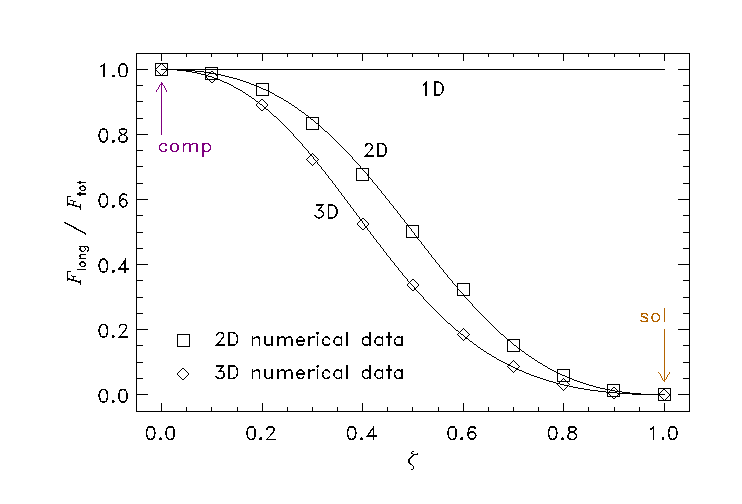
\includegraphics[width=0.6\linewidth]{federrath_stirring_ratio}}
\caption{Ratio of compressive to total power of the turbulent stirring field, reprinted from Federrath
et al.~(2010, A\&A, 512, A81) with permission by Astronomy \& Astrophysics. The solid lines labelled
with 1D, 2D, and 3D show the analytical expectation for this ratio, equation~(\ref{eq:forcing_ratio}),
as a function of the stirring parameter $\zeta$ for one-, two- and three-dimensional driving,
respectively. The diamonds and squares show results of numerical simulations in 3D and 2D with
$\zeta=[0,1]$, separated by $\Delta\zeta=0.1$. The two limiting cases of purely solenoidal stirring
($\zeta=1$) and purely compressive stirring ($\zeta=0$) are indicated as ''sol'' and ''comp'',
respectively. Note that in any 1D model, all power is in the compressive component, and thus
$F_\mathrm{long}/F_\mathrm{tot}=1$, independent of $\zeta$.}
\label{fig:federrath_stirring_ratio}
\end{figure*}

The second term on the right-hand side of equation~(\ref{eq:ou}) is a drift term describing the
exponential decay of the autocorrelation of $\vec{f}$. The usual procedure is to set the autocorrelation
timescale equal to the turbulent crossing time, $T=L_\mathrm{peak}/V$, on the scale of energy injection,
$L_\mathrm{peak}$. This type of stirring models the kinetic energy input from large-scale turbulent
fluctuations breaking up into smaller and smaller structures.

The runtime parameters associated with the \code{StirFromFile} unit are described in the
\ref{Sec:StirFromFileUnitUsing} section.


\subsection{Using the StirFromFile Unit}
\label{Sec:StirFromFileUnitUsing}

\subsubsection{Runtime Parameters}

\begin{table}[ht]
\caption{Runtime parameters for the stirring module.} \label{tab:federrath_stirring}
\begin{center}
\begin{tabular}{lllp{18em}}
Variable & Type & Default & Description \\
\hline 
\rpi{Stir/useStir} & boolean & .true. & switch stirring on/off \\
\rpi{Stir/st\_computeDt} & boolean & .false. & restrict timestep based on stirring \\
\rpi{Stir/st\_infilename} & string & "forcingfile.dat" & file containing the stirring time sequence \\
\hline
\end{tabular}
\end{center}
\end{table}

Table~\ref{tab:federrath_stirring} lists the runtime parameters for the StirFromFile unit. This
includes a switch for turning the stirring module on/off and a switch to restrict the timestep based
on the acceleration field used for stirring (\rpi{Stir/st\_computeDt} is switched off by default, because
it is normally sufficient to restrict the timestep based on the gas velocity). Finally,
\rpi{Stir/st\_infilename} is the name of the input file containing the time and mode sequence used for
stirring. This file must be prepared in advance with a separate Fortran program located in
\code{SimulationMain/StirFromFile/forcing_generator/}. The reason for this structural splitting
is to predetermine what the code is going to do. For instance, by preparing the time sequence of
the stirring in advance, one can always reproduce exactly the full evolution of all driving patterns
applied during a simulation. It also has the advantage that exactly identical stirring patterns can
be applied in completely different codes, because they read the time and mode sequence from the same
stirring file (Price \& Federrath, 2010, MNRAS, 406, 1659).

The stirring module is compatible with any hydro or MHD solver and any grid implementation (uniform
or AMR). Upon inclusion in a Flash-X setup or module, the \code{StirFromFile} module defines three
additional grid scalar fields, \code{accx}, \code{accy}, and \code{accz}, holding the three vector
components of the stirring field $\vec{f}$.


\subsubsection{Preparing the Stirring Sequence (\code{st\_infilename})}
\label{sec:federrath_prepare_stir}

\begin{table}[ht]
\caption{Parameters in \code{forcing\_generator.F90} to prepare a stirring sequence.}
\label{tab:federrath_forcing_generator}
\begin{center}
\begin{tabular}{lllp{24em}}
Variable & Type & Default & Description \\
\hline 
\texttt{ndim} & integer & $3$ & The dimensionality of the simulation (1, 2, or 3) \\
\texttt{xmin, xmax} & real & $-0.5,\,0.5$ & Domain boundary coordinates in $x$ direction \\
\texttt{ymin, ymax} & real & $-0.5,\,0.5$ & Domain boundary coordinates in $y$ direction \\
\texttt{zmin, zmax} & real & $-0.5,\,0.5$ & Domain boundary coordinates in $z$ direction \\
\texttt{st\_spectform} & integer & $1$ & Spectral shape (0:~band, 1:~paraboloid) \\
\texttt{st\_decay} & real & $0.5$ & Autocorrelation time of the OU process, $T=L_\mathrm{peak}/V$ \\
\texttt{st\_energy} & real & 2e-3 & Determines the driving amplitude \\
\texttt{st\_stirmin} & real & $6.283$ & Minimum wavenumber stirred (e.g., $k_\mathrm{min}\lesssim2\pi/L_\mathrm{box}$) \\
\texttt{st\_stirmax} & real & $18.95$ & Maximum wavenumber stirred (e.g., $k_\mathrm{max}\gtrsim6\pi/L_\mathrm{box}$) \\
\texttt{st\_solweight} & real & $1.0$ & Mode mixture $\zeta=[0,1]$ in Eq.~(\ref{eq:forcing_ratio}).
Typical values are $1.0$:~solenoidal; $0.0$:~compressive; $0.5$:~natural mixture. \\
\texttt{st\_seed} & integer & $140281$ & Random seed for stirring sequence \\
\texttt{end\_time} & real & $5.0$ & Final time in stirring sequence \\
\texttt{nsteps} & integer & $100$ & Number of realizations between $t=0$ and \code{end\_time} \\
\texttt{outfilename} & string & "forcingfile.dat" & Output name (input file \code{st\_infilename} for Flash-X) \\
\hline
\end{tabular}
\end{center}
\end{table}

The code requires a time sequence of stirring modes at runtime, which have to be prepared with the
stand-alone Fortran program \code{forcing\_generator.F90} in \code{SimulationMain/StirFromFile/forcing_generator/}.
A Makefile is provided in the same directory. This program prepares the time sequence of Fourier modes,
which is then read by Flash-X during runtime, to construct the physical acceleration fields used for stirring.
It controls the spatial structure and the temporal correlation of the driving, its amplitude, the mode mixture,
and the time separation between successive driving patterns. The user has to modify \code{forcing_generator.F90}
to construct a requested driving sequence and to tailor it to the desired physical situation to be modeled.

Table~\ref{tab:federrath_forcing_generator} lists all the parameters that can be adjusted in the main routine
of \code{forcing\_generator.F90}. Most of them are straightforward to set (\code{ndim},
\code{xmin, xmax, ymin, ...}\footnote{Note that we typically assume a cubic box with side length
$L_\mathrm{box}=\code{xmax}-\code{xmin}=\code{ymax}-\code{ymin}=\code{zmax}-\code{zmin}$}), but others
may require some explanation. For example, \code{st\_spectform} determines the shape of the driving amplitude
in Fourier space. Many colleagues drive a band (\code{st\_spectform}=0), i.e., equal power injected between
wavenumber modes $k_\mathrm{min}=\code{st\_stirmin}$ and $k_\mathrm{max}=\code{st\_stirmax}$. This produces a
sharp transition between stirred modes and modes that are not stirred. Here we set the default to a smooth
function, a paraboloid (\code{st\_spectform}=1), such that most power is injected on wavenumber
$k_\mathrm{peak}=(k_\mathrm{min}+k_\mathrm{max})/2$ and falls off quadratically towards both wavenumber ends,
normalized such that the injected power at $k_\mathrm{min}$ and $k_\mathrm{max}$ vanishes. This has the
advantage of defining a characteristic peak injection scale $k_\mathrm{peak}$ and achieves a smooth transition
between stirred and non-stirred wavenumbers.

\code{st\_decay} and \code{st\_energy} determine the autocorrelation time of the OU process and the total injected
energy, which is simply a measure for the normalization of the acceleration field. These parameters must be
adjusted according to the physical setup. For instance, for a given target velocity dispersion $V$ on the injection
scale $L_\mathrm{peak}=2\pi/k_\mathrm{peak}$, the autocorrelation time should be set equal to the turbulent crossing
time, $T=L_\mathrm{peak}/V$. In contrast, setting \code{st\_decay} to a very small or a very large number results
in white noise driving or in a static driving pattern, respectively.

The parameter \code{st\_solweight} determines whether the acceleration field will be solenoidal (divergence-free)
or compressive (curl-free) or any mixture, according to Equation~(\ref{eq:forcing_ratio}). Incompressible gases
should naturally be driven with a purely solenoidal field ($\zeta=1$), while compressible turbulence in the
interstellar medium may be driven primarily by a mixture of solenoidal and compressive modes. A detailed study
of the influence of $\zeta$ is presented in Federrath et al.~(2010, A\&A, 512, A81).

\code{st\_seed} is the random seed for the OU sequence and determines the pseudo random number sequence for the
integrated Box-Muller random number generator.

Finally, \code{end\_time} and \code{nsteps} determine the final physical time for stirring and the number of
driving patterns to be prepared within the time period from $t=0$ to $t=\code{end\_time}$. This sets the number
of equally-spaced times at which Flash-X is going to read a new stirring pattern from the file. This allows the
user to control how frequently a new driving pattern is constructed. A useful time separation of successive
driving patterns is about 10\% of a crossing time (or autocorrelation time), i.e., setting
$\code{nsteps}=10\times\code{end\_time}/\code{st\_decay}$. This will sample the smooth changes in the OU
driving sequence sufficiently well for most applications.


\subsection{Stirring Unit Test}

An example setup using the \code{StirFromFile} unit is located in \code{SimulationMain/StirFromFile/}.
The unit test can be invoked by

\code{./setup StirFromFile -auto -3d -nxb=16 -nyb=16 -nzb=16 +ug -with-unit=physics/Hydro}.

\noindent
The Flash-X executable must be copied into the run directory together with the standard \code{flash.par}
for this setup, and together with the default forcing file (to be constructed using the standard parameters;
see section~\ref{sec:federrath_prepare_stir}). During runtime the code writes a file with the time evolution
of spatially integrated quantities, amongst others, the rms Mach number and vorticity, which can used as
basic code checks.



%\input{sourceTerms-chf-Summer2013}  (old version)


\begin{comment}
\section{Heating Unit}
\label{Sec:heating}

\subsection{Static + Gaussian heating}
\label{Sec:stat+gauss}

The \code{source\_terms/heat/stat+gauss} unit implements a
phenomenological heating term of the plasma parameterized as a function
of position and time.  The specific implementation assumes that the
heating function consists of the sum of two terms --  a steady, uniform
term $Q_0$ and a transient heating $Q_i(\avec{s},t)$, prescribed as
a separable function of spatial coordinates and time
\begin{equation}
Q_i(\avec{s}, t) = H_0 \times g(\avec{s}) \times f(t)~.
\end{equation}
where $H_0$ is the peak value of the heating rate, $g(\avec{s})$ is
the distribution along the spatial coordinate $\avec{s} \equiv [x,y,z]$,
in our case a 3-D Gaussian function,
\begin{equation}
g(\avec{s}) = \exp[-(\avec{s}-\avec{s}_0)^2 / 2\sigma^2]~,
\end{equation}
and f(t) is prescribed as a step function of time followed by an
exponential decrease, \ie,
\begin{equation}
f(t) = \left\{ \begin{array}{l@{\quad}l}
                0,  & t \le t^* \\
                1,  & t^* < t \le t_0 ~~,\\
                \exp[(t_0-t)/\tau], & t > t_0
                 \end{array} \right.
\end{equation}
where $t^*$ is the beginning of the impulsive heating phase.

\subsection{Usage}
\label{Sec:stat+gauss usage} The runtime parameters used with
the \code{stat+gauss} unit are summarized in
\tblref{Tab:stat+gauss parameters}.


\begin{center}
\begin{longtable}{lllp{3in}}
\caption{ \label{Tab:stat+gauss parameters} Runtime parameters for the
\code{stat+gauss} unit.} \\
%\begin{tabular}{lllp{3in}}

Variable        & Type          & Default & Description\\

\hline
\code{statheat}     & real       & $1.0\times10^{-5}$       &
                           Stationary heating $({\rm erg~cm}^{-3} s^{-1})$ \\

\code{qheat}   & real  & 0.0       & Peak value of the transient heating
rate (erg cm$^{-3}$ s$^{-1}$)\\

\code{x0heat}  & real          & 1.0 & X location (cm) of the transient
heating \\
\code{y0heat}  & real          & 1.0 & Y location (cm) of the transient
heating \\
\code{z0heat}  & real          & 1.0 & Z location (cm) of the transient
heating \\
\code{sigheat}  & real          & 1.0& Sigma (cm) of the transient
heating \\

\code{tstar}  & real          & -1.0      & Time (s) of beginning of the impulsive heating phase \\

\code{t0heat}& real          & -1.0    & Switch off time (s) of the transient heating\\

\code{tau}& real          & 1.0    & Decay time (s) of the transient heating\\
\code{theatmin} & real    & $1.0\times10^{3}$  & Minimum temperature (K) allowed in the \code{stat+gauss} unit\\

\hline
%\end{tabular}
\end{longtable}
\end{center}

\section{Cooling Unit}
\label{Sec:cooling}

\subsection{Radiative losses from an optically thin plasma}
\label{Sec:radloss}

The \code{source\_terms/cool/radloss} unit implements radiative
losses from an optically thin plasma.
The radiative losses per unit emission $\Lambda(T)$ measured from an
optically thin plasma
(Raymond and Smith, 1977, Raymond 1978) have been implemented
adopting a piecewise-power law approximation that provides a reasonable
fit to $\Lambda(T)$.  The expression adopted is given by Rosner,
Tucker and Vaiana (1978) to model the energy losses from the transition region
and corona in the temperature range
\begin{equation}
\label{Eqn:transition and corona energy losses}
2 \times 10^{4} < T < 10^{8} K
\end{equation}
and by Peres {\it et al.} (1982) to model the energy losses from the
chromosphere in the range
\begin{equation}
\label{Eqn:chromosphere energy losses}
4.44 \times 10^{3} < T < 2 \times 10^{4} K~.
\end{equation}
The resulting formulation is as follows:
\begin{equation}
\Lambda(T) =
   \left\{ \begin{array}{l@{\quad}l}
   (10^{-5.97} T)^{11.7}  & 10^{3.65} {\rm\ K} < T <  10^{3.9} {\rm\ K}\\
   (10^{-7.85} T)^{6.15}  & 10^{3.9} {\rm\ K} < T <  10^{4.3} {\rm\ K}\\
   10^{-21.85}            & 10^{4.3} {\rm\ K} < T <  10^{4.6} {\rm\ K}\\
   10^{-31} T^{2}         & 10^{4.6} {\rm\ K} < T <  10^{4.9} {\rm\ K}\\
   10^{-21.2}             & 10^{4.9} {\rm\ K} < T <  10^{5.4} {\rm\ K}\\
   10^{-10.4} T^{-2}      & 10^{5.4} {\rm\ K} < T <  10^{5.75} {\rm\ K}\\
   10^{-21.94}            & 10^{5.75} {\rm\ K} < T <  10^{6.3} {\rm\ K}\\
   10^{-17.73} T^{-2/3}   & 10^{6.3}  {\rm\ K} < T <  10^{7}   {\rm\ K}\\
   10^{-18.21} T^{-0.6}   & 10^{7}    {\rm\ K} < T <  10^{7.6} {\rm\ K}\\
   10^{-26.57} T^{1/2}    & 10^{7.6}  {\rm\ K} < T <  10^{8}   {\rm\ K}
   \end{array} \right.
\end{equation}

\subsection{Usage}\label{Sec:radloss usage}

The runtime parameters used with the \code{radloss} unit are
summarized in \tblref{Tab:radloss parameters}. The unit requires
the use of a fluid composition containing at least protons and
electrons.  The composition unit \texttt{
materials/composition/prot+elec} and the units in \texttt{
materials/composition/ioniz} satisfy this condition.

\begin{center}
\begin{longtable}{lllp{3in}}
\caption{\label{Tab:radloss parameters}Runtime parameters used with the \code{
radloss} unit.} \\

%\begin{tabular}{lllp{3in}}

Variable        & Type          & Default       & Description\\
\hline
\code{tradmin}  & REAL          & $4.44\times10^3$    & Minimum temperature (K)
                                           allowed in the \code{radloss} unit\\
\code{tradmax}   & REAL          & $1.1\times10^8$    & Maximum temperature (K)
                                                  allowed in the unit\\
\code{dradmin}   & REAL          & 1.0         & Minimum electron number
                                                  density (cm$^{-3}$) allowed
                                                  in the unit\\
\code{dradmax}   & REAL      & $1.0\times10^{14}$     & Maximum electron number
                                       density (cm$^{-3}$) allowed in the unit\\
\hline
%\end{tabular}
\end{longtable}
\end{center}
\end{comment}




% \input{EnergyDeposition}
% \input{Heatexchange}
% \input{Flame}
